% Dokumentklassen s�ttes til memoir.
% Manual: http://ctan.org/tex-archive/macros/latex/contrib/memoir/memman.pdf
\documentclass[a4paper,oneside,article]{memoir}

\usepackage{pgf}
\usepackage{tikz}
\usepackage{pgfplots}
\usetikzlibrary{arrows,automata}
\usepackage{verbatim}
 
% Danske udtryk (fx figur og tabel) samt dansk orddeling og fonte med
% danske tegn. Hvis LaTeX brokker sig over �, � og � skal du udskifte
% "utf8" med "latin1" eller "applemac". 
\usepackage{inputenc}
\usepackage[danish]{babel}
\usepackage[T1]{fontenc}
 
% Matematisk udtryk, fede symboler, theoremer og fancy ting (fx k�debr�ker)
\usepackage{amsmath,amssymb}
\usepackage{bm}
\usepackage{amsthm}
%\usepackage{mathtools}
 
% Kodelisting. Husk at l�se manualen hvis du vil lave fancy ting.
% Manual: http://mirror.ctan.org/macros/latex/contrib/listings/listings.pdf
\usepackage{listings}
 
% Fancy ting med enheder og datatabeller. L�s manualen til pakken
% Manual: http://www.ctan.org/tex-archive/macros/latex/contrib/siunitx/siunitx.pdf
%\usepackage{siunitx}

% Inds�ttelse af grafik.
\usepackage{graphicx}
\usepackage{float}
\usepackage{caption}
\usepackage{subcaption}
 
% Reaktionsskemaer. L�s manualen for at se eksempler.
% Manual: http://www.ctan.org/tex-archive/macros/latex/contrib/mhchem/mhchem.pdf
%\usepackage[version=3]{mhchem}
%\usepackage[noend]{algpseudocode}
%\usepackage{algorithm}

\usepackage{xcolor,colortbl}

\usepackage{listings}

\definecolor{javared}{rgb}{0.6,0,0} % for strings
\definecolor{javagreen}{rgb}{0.25,0.5,0.35} % comments
\definecolor{javapurple}{rgb}{0.5,0,0.35} % keywords
\definecolor{javadocblue}{rgb}{0.25,0.35,0.75} % javadoc

\lstset{language=Java,
basicstyle=\small, %\ttfamily,
keywordstyle=\color{javapurple}\bfseries,
stringstyle=\color{javared},
commentstyle=\color{javagreen},
morecomment=[s][\color{javadocblue}]{/**}{*/},
numbers=left,
numberstyle=\tiny\color{black},
stepnumber=1,
numbersep=10pt,
tabsize=4,
showspaces=false,
showstringspaces=false}

\newcommand{\notimplies}{%
  \mathrel{{\ooalign{\hidewidth$\not\phantom{=}$\hidewidth\cr$\implies$}}}}

\begin{document}
    \title{Distributed Commit - Disposition}
    \author{Lukas Peter J�rgensen, 201206057, DA4
            }
    \maketitle
    
    \chapter{Introduction}
    \section*{Goals:}
    Given a process group and an operation, if the operation is committable at all processes, commit at all processes.\\
    Either everybody eventually commits or everybody eventually aborts, even crashed servers.
    
    \section*{One-phase commit}
    A coordinator tells all other processes whether ot not to perform the operation question.\\
    \textbf{Drawback:} If a process cannot perform the operation, there is no way to tell the coordinator.
    
    \section*{Two-phase commit}
    \begin{enumerate}
    \item Coordinator sends a VOTE\_REQUEST message to all participants.
    \item When a participant receives a VOTE\_REQUEST, it returns either COMMIT or ABORT.
    \item Coordinator collects all votes from the participants, if everyone voted COMMIT, then so will the coordinator. Then it sends a GLOBAL\_COMMIT to everyone otherwise it sends GLOBAL\_ABORT.
    \item Each participant waits for the final reaction, and acts accordingly.
    \end{enumerate}
    
    \begin{figure}[H]
    \centering
    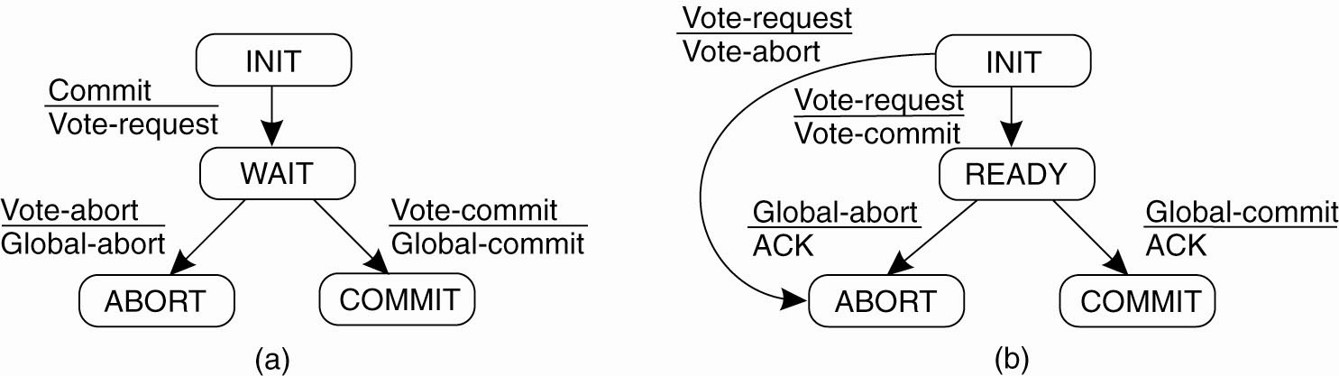
\includegraphics[width=\textwidth]{Media/2PCommit.jpg}
    \end{figure}
    
    \subsection*{Problems}
    Several problems arise if the 2PC protocol is used in a system where failures occur.\\
    Timeout mechanisms needed to prevent a process from blocking all the other processes.\\
    \\
    \textbf{Participants in INIT waiting for VOTE\_REQUEST}, if that message is not received after some time, the participant will simply decide to locally abort the transaction, and thus send an ABORT message.\\
    \\
    \textbf{Coordinator in WAIT, waiting for the votes}, if not all votes have been collected after some time, send GLOBAL\_ABORT.\\
    \\
    \textbf{Participants in READY state waiting for global vote}, if that message is not received within a given time, it cannot simply abort transaction. It can either wait for the coordinator, or consult other participants.\\
    \\
    \textbf{Logging:} 2PC handles crashes by logging the state to a permanent storage.
    \subsection*{Conclusion}
    Two-phase commit has the problem that if the coordinator or one participant crashes at a bad time, it will freeze the entire system untill they are up and running again.
    
    \section*{Three-phase commit}
    \begin{figure}[H]
    \centering
    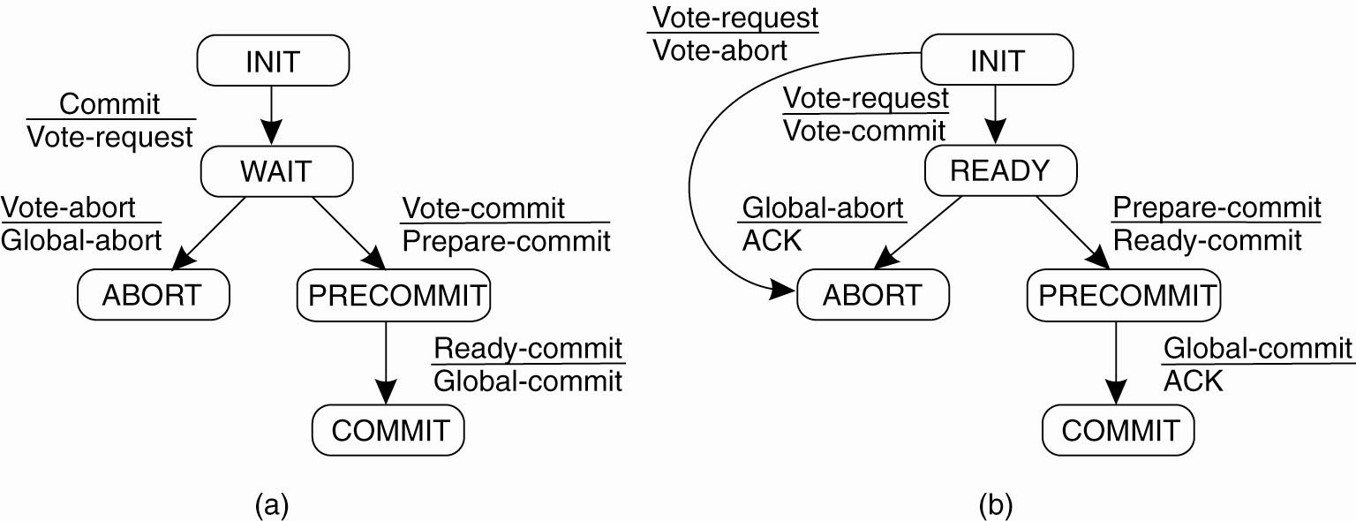
\includegraphics[width=\textwidth]{Media/3PCommit.jpg}
    \end{figure}
        
    Enhances two-phase commit, by being non-blocking in more cases.\\
    As long as the live participants can make a majority decision among both live and dead participants, they can continue on their own.\\
    Very unlikely to block if there are many participants.
    \\
    \\
    \textbf{IF} anyone else in ABORT $\rightarrow$ ABORT.
    \textbf{ELIF} anyone else in COMMIT $\rightarrow$ COMMIT.
    \textbf{ELIF} anyone else in INIT $\rightarrow$ ABORT.
    \textbf{ELSE} everyone else in READY or PRECOMMIT, do a majority vote.
    
\end{document}